\includeonlyframes{current}

\begin{frame}
  \frametitle{C/\cpp origins}
  \begin{minipage}{0.4\linewidth}
    \tikzstyle{old}=[ellipse,draw=black,fill=orange!30,thick,inner sep=2pt]
    \tikzstyle{new}=[rectangle,draw=black,fill=green!50,thick,inner sep=2pt]
    \tikzstyle{direct}=[<-,semithick]
    \tikzstyle{transverse}=[<-,dotted,semithick]
    \begin{tikzpicture}[->, node distance=.75cm, font=\tiny]
      \node[old] (Simula)      {Simula};
      \node[left of=Simula,node distance=1.5cm] {1967};
      \node[old] (BCPL) [right of=Simula, node distance=2cm] {BCPL};
      \node[old] (B) [below of=BCPL] {B}
      edge[transverse] (BCPL);
      \node[old] (KandRC) [below of=B] {K and R C}
      edge[transverse] (B);
      \node[left of=KandRC,node distance=3.5cm] {1978};
      \node[old] (ClassicC) [below of=KandRC] {Classic C}
      edge[direct] (KandRC);
      \node[old] (CwithClasses) [below of=Simula,node distance=3cm] {C with Classes}
      edge[transverse] (Simula)
      edge[transverse] (BCPL)
      edge[direct] (ClassicC);
      \node[left of=CwithClasses,node distance=1.5cm] {1980};
      \node[old] (EarlyC++) [below of=CwithClasses] {Early \cpp}
      edge[direct] (CwithClasses);
      \node[left of=EarlyC++,node distance=1.5cm] {1985};
      \node[old] (C89) [below of=ClassicC,node distance=2.25cm] {C89}
      edge[direct] (ClassicC)
      edge[transverse] (CwithClasses);
      \node[old] (ARMC++) [below of=EarlyC++] {ARM \cpp}
      edge[direct] (EarlyC++)
      edge[transverse] (C89);
      \node[left of=ARMC++,node distance=1.5cm] {1989};
      \node[old] (C++98) [below of=ARMC++] {\cpp98}
      edge[direct] (ARMC++)
      edge[transverse] (C89);
      \node[old] (C99) [below of=C89] {C99}
      edge[direct] (C89)
      edge[transverse] (ARMC++);
      \node[left of=C++98,node distance=1.5cm] {1998};
      \node[new] (C++11) [below of=C++98] {\cpp11}
      edge[direct] (C++98)
      edge[transverse] (C99);
      \node[left of=C++11,node distance=1.5cm] {2011};
      \node[new] (C11) [below of=C99] {C11}
      edge[direct] (C99)
      edge[transverse] (C++98);
      \node[new] (C++14) [below of=C++11] {\cpp14}
      edge[direct] (C++11);
      \node[left of=C++14,node distance=1.5cm] {2014};
    \end{tikzpicture}
  \end{minipage}
  \begin{minipage}{0.57\linewidth}
    \begin{tabular}{cc}
      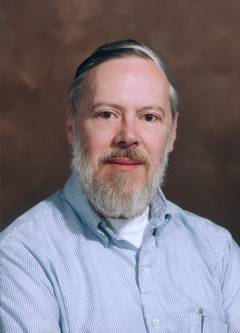
\includegraphics[height=2.5cm]{ritchie.jpeg} & 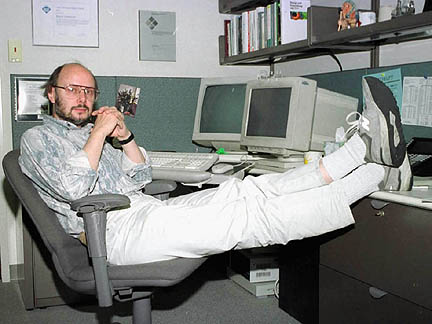
\includegraphics[height=2.5cm]{BjarneStroustrup.jpg} \\[-1ex]
      \tiny{C inventor} & \tiny{\cpp inventor} \\[-1ex]
      \scriptsize{Dennis M. Ritchie} & \scriptsize{Bjarne Stroustrup} \\
    \end{tabular}
    \begin{itemize}
      {\footnotesize
      \item Both C and \cpp are born in Bell Labs
      \item \cpp \it{almost} embeds C
      \item C and \cpp are still under development
      \item we will mainly discuss \cpp98
      }
    \end{itemize}
  \end{minipage}
\end{frame}

\subsubsection{Does it fit our needs ?}

\begin{frame}
  \frametitle{Why ic \cpp our language of choice ?}
  \pause
  \begin{block}{Adapted to large projects}
    \begin{itemize}
    \item strongly typed
    \item object oriented
    \item many available libraries
    \end{itemize}
  \end{block}
  \pause
  \begin{block}{Fast}
    \begin{itemize}
    \item as it's compiled (unlike Java or C\#)
    \item allows to go close to hardware
    \end{itemize}
  \end{block}
\end{frame}

\subsection[Basics]{Langage basics}

\begin{frame}[fragile]
  \frametitle{Hello World}
  preprocessor, functions, ;, for, decl,...
  \begin{cppcode}
    #include <iostream>

    // This is a function
    void print(int i) {
      std::cout << "Hello, world " << i << std::endl;
    }

    int main(int argc, char** argv) {
      int n = 3;
      for (int i = 0; i < n; i++) {
        print(i);
      }
      return 0;
    }
  \end{cppcode}
\end{frame}

\begin{frame}[fragile]
  \frametitle{Comments}
  \begin{cppcode}
    // simple comment for integer declaration
    int i;

    /* multiline comment
     * in case we need to say more
     */
    double d;

    /**
     * Best choice : doxygen compatible comments
     * \fn bool isOdd(int i)
     * \brief checks whether i is odd
     * \param i input
     * \return true if i is odd, otherwise false
     */
     bool isOdd(int i);
  \end{cppcode}
\end{frame}

\begin{frame}[fragile]
  \frametitle{Basic types(1)}
  \begin{cppcode}
    bool b = true;            // boolean, true or false
    
    char c = 'a';             // 8 bits ASCII char
    char* s = "a C string";   // array of chars ended by \0
    string t = "a C++ string";// class provided by the STL

    char c = -3;              // 8 bits signed integer
    unsigned char c = 4;      // 8 bits unsigned integer

    short int s = -444;       // 16 bits signed integer
    unsigned short s = 444;   // 16 bits unsigned integer
    short s = -444;           // int is optionnal
  \end{cppcode}
\end{frame}
\begin{frame}[fragile]
  \frametitle{Basic types(2)}
  \begin{cppcode}
    int i = -123456;          // 32 bits signed integer
    unsigned int i = 1234567; // 32 bits signed integer

    long l = 0L               // 32 or 64 bits (ptr size)
    unsigned long l = 0UL;    // 32 or 64 bits (ptr size)

    long long ll = 0LL;       // 64 bits signed integer
    unsigned long long l = 0ULL; // 64 bits unsigned integer

    float f = 1.23;           // 32 (23+7+1) bits float
    double d = 1.23E34;       // 64 (52+11+1) bits float
  \end{cppcode}
\end{frame}

\begin{frame}[fragile]
  \frametitle{Portable numeric types}
  \alert{One needs to include specific header}
  \begin{cppcode}
    #include <stdint.h>
    
    int8_t c = -3;     // 8 bits, replaces char
    uint8_t c = 4;     // 8 bits, replaces unsigned char

    int16_t s = -444;  // 16 bits, replaced short
    uint16_t s = 444;  // 16 bits, replaced unsigned short

    int32_t s = -0674; // 32 bits, replaced int
    uint32_t s = 0674; // 32 bits, replaced unsigned int

    int64_t s = -0x1bc;// 64 bits, replaced long long
    uint64_t s = 0x1bc;// 64 bits, replaced unsigned long long
    \end{cppcode}
\end{frame}

\begin{frame}[fragile]
  \frametitle{Static arrays}
  \begin{cppcode*}{}
    int ai[4] = {1,2,3,4};
    int ai[] = {1,2,3,4};  // identical
    
    char ac[3] = {'a','b','c'};   // char array
    char ac[4] = "abc";           // valid C string
    char ac[4] = {'a','b','c',0}; // same valid string
    
    int i = ai[2];  // i = 3
    char c = ac[8]; // garbage
    int i = ai[4];  // also garbage !
  \end{cppcode*}
\end{frame}

\begin{frame}[fragile]
  \frametitle{Pointers}
  \begin{multicols}{2}
    \begin{cppcode*}{gobble=6}
      int i = 4;
      int *pi = &i;
      int j = *pi + 1;
      
      int ai[] = {1,2,3};
      int *pai = ai;
      int *paj = pai + 1;
      int k = *paj + 1;
      
      int *pak = k;
      int *pak = (int*)k;
      int l = *pak; // seg fault !
    \end{cppcode*}
    \onslide<2->{
      \begin{tikzpicture}
        \memorystack[size x=3cm,word size=1,nb blocks=11]
        \onslide<3-> {\memorypush{$i = 4$}}
        \onslide<4-> {\memorypushpointer[pi =]{1}}
        \onslide<5-> {\memorypush{$j = 5$}}
        \onslide<6-> {\memorypush{$1$}}
        \onslide<6-> {\memorypush{$2$}}
        \onslide<6-> {\memorypush{$3$}}
        \onslide<6-> {\memorypushpointer[ai =]{4}}
        \onslide<7-> {\memorypushpointer[pai =]{4}}
        \onslide<8-> {\memorypushpointer[paj =]{5}}
        \onslide<9-> {\memorypush{$k = 3$}}
        \onslide<10-> {\memorypush{$pak = 3$}}
        \onslide<10-> {\draw[\stackcolor!80,->] (stack11-1.west) -- +(-0.5cm,0)
          node [anchor=east] {??};}
      \end{tikzpicture}
    }
  \end{multicols}
\end{frame}

\begin{frame}[fragile]
  \frametitle{Dynamic Arrays}
  \begin{cppcode*}{}
    #include <stdlib.h>
    #include <string.h>

    int *ai;     // pointer to random address
    int *ai = 0; // better. Can be tested

    // allocate array of 10 ints (not initialized)
    ai = (int*) malloc(10*sizeof(int));
    // and set them to 0
    memset(ai, 10, sizeof(int));

    // Both in one go
    ai = (int*) calloc(10, sizeof(int));
    
    // liberate memory
    free(ai);
  \end{cppcode*}
\end{frame}

\begin{frame}[fragile]
  \frametitle{Operators(1)}
  \begin{block}{Binary \& Assignment Operators}
    \begin{cppcode*}{linenos=false,gobble=4}
      int i = 1 + 4 - 2;  // 3
      i *= 3;             // 9
      i /= 2;             // 4
      i = 23 % i;         // modulo => 3
    \end{cppcode*}
  \end{block}
  \pause
  \begin{block}{Increment / Decrement \uncover<3->{\hfill \alert{\bf Use wisely}}}
    \begin{cppcode*}{linenos=false}
      int i = 0; i++; // i = 1
      int j = ++i;    // i = 2, j = 2
      int k = i++;    // i = 3, k = 2
      int l = --i;    // i = 2, l = 2
      int m = i--;    // i = 1, m = 2
    \end{cppcode*}
  \end{block}
\end{frame}

\begin{frame}[fragile]
  \frametitle{Operators(2)}
  \begin{block}{Bitwise and Assignment Operators}
    \begin{cppcode*}{linenos=false,gobble=4}
      int i = 0xee & 0x55;  // 0x44
      i |= 0xee;            // 0xee
      i ^= 0x55;            // 0xbb
      int j = ~0xee;        // 0xffffff11
      int k = 0x1f << 3;    // 0x78
      int l = 0x1f >> 2;    // 0x7
    \end{cppcode*}
  \end{block}
  \pause
  \begin{block}{Boolean Operators}
    \begin{cppcode*}{linenos=false,gobble=4}
      bool a = true;
      bool b = false;
      bool c = a && b;    // false
      bool d = a || b;    // true
      bool e = !d;        // false
    \end{cppcode*}
  \end{block}
\end{frame}

\begin{frame}[fragile]
  \frametitle{Operators(3)}
  \begin{block}{Comparison Operators}
    \begin{cppcode*}{linenos=false,gobble=4}
      bool a = (3 == 3);  // true
      bool b = (3 != 3);  // false
      bool c = (4 < 4);   // false
      bool d = (4 <= 4);  // true
      bool e = (4 > 4);   // false
      bool f = (4 >= 4);  // true
    \end{cppcode*}
  \end{block}
  \pause
  \begin{block}{Precedences \uncover<3->{\hfill \alert{\bf Don't use}\uncover<4->{\color{green} \bf\ - use parenthesis}}}
    \begin{cppcode*}{linenos=false}
      c &= 1+(++b)|(a--)*4%5^7; // ???
    \end{cppcode*}
  \end{block}
\end{frame}

\begin{frame}[fragile,label=current]
  \frametitle{struct}
  \begin{mdframed}[style=simplebox]
    \center ``members'' grouped together under one name
  \end{mdframed}
  \begin{multicols}{2}
    \begin{cppcode*}{gobble=6}
      struct Individual {
        unsigned char age;
        float weight;
      };

      Individual student;
      student.age = 25;
      student.weight = 78.5;
    \end{cppcode*}
    \columnbreak
    \begin{cppcode*}{gobble=6,firstnumber=9}
      Individual teacher = {
        .age = 45,
        .weight=67
      };
    \end{cppcode*}
    \pause
    \null \vfill
    \begin{tikzpicture}
      \memorystack[nb blocks=5]
      \onslide<4-> {
        \memorypush{25,?,?,?}
        \memorypush{7,8,.,5}
        \memorystruct{1}{2}{\scriptsize student}
      }
      \onslide<5-> {
        \memorypush{45,?,?,?}
        \memorypush{6,7,.,0}
        \memorystruct{3}{4}{\scriptsize teacher}
      }
    \end{tikzpicture}
    \vfill \null
  \end{multicols}
\end{frame}

\begin{frame}[fragile]
  \frametitle{union}
  \begin{mdframed}[style=simplebox]
    \center ``members'' packed together at same memory location
  \end{mdframed}
  \begin{multicols}{2}
    \begin{cppcode*}{gobble=6}
      union Duration {
        int seconds;
        short hours;
        char days;
      };

      Duration d1, d2, d3;
      d1.seconds = 259200;
      d2.hours = 72;
      d3.days = 3;
      d1.days = 3; // d1.seconds overwritten
      int a = d1.seconds; // d1.seconds is garbage
    \end{cppcode*}
    \pause
    \columnbreak
    \null \vfill
    \onslide<2->{
      \begin{tikzpicture}
        \memorystack[word size=1,nb blocks=4]
        \visible<3-5>{\memorypush{d1.seconds=259200}}
        \onslide<4->{\memorypush{d2.hours=259200}}
        \onslide<5->{\memorypush{d3.days=3}}
        \memorygoto{1}
        \onslide<6->{\memorypush{d1.days=3}}
      \end{tikzpicture}
    }
    \vfill \null
  \end{multicols}
\end{frame}

\begin{frame}[fragile]
  \frametitle{Enums and typedefs}
  \begin{multicols}{2}
    \begin{cppcode*}{gobble=6}
      enum VehicleType {
        BIKE,  // 0
        CAR,   // 1
        BUS,   // 2
      };
      VehicleType t = CAR;
      
      typedef uint64_t myint;
      myint toto = 17;
    \end{cppcode*}
    \columnbreak
    \begin{cppcode*}{gobble=6}
      enum VehicleType {
        BIKE = 3,
        CAR = 5,
        BUS = 7,
      };
      VehicleType t2 = BUS;
    \end{cppcode*}
  \end{multicols}
\end{frame}


\begin{frame}[fragile]
  \frametitle{More sensible example}
  \begin{multicols}{2}
    \begin{cppcode*}{gobble=6}
      enum ShapeType {
        CIRCLE,
        RECTANGLE
      };
      
      struct Rectangle {
        float width;
        float height;
      };
    \end{cppcode*}
    \columnbreak
    \pause
    \begin{cppcode*}{gobble=6,firstnumber=10}
      struct Shape {
        ShapeType type;
        union { 
          float radius;
          Rectangle rect;
        };
      };
    \end{cppcode*}
  \end{multicols}
  \pause
  \begin{multicols}{2}
    \begin{cppcode*}{gobble=6,firstnumber=17}
      Shape s;
      s.type = CIRCLE;
      s.radius = 3.4;
      
    \end{cppcode*}
    \columnbreak
    \begin{cppcode*}{gobble=6,firstnumber=20}
      Shape t;
      t.type = RECTANGLE;
      t.rect.width = 3;
      t.rect.height = 4;
    \end{cppcode*}
  \end{multicols}
\end{frame}

\begin{frame}[fragile]
  \frametitle{Functions}
  \begin{multicols}{2}
    \begin{cppcode*}{gobble=6}
      // with return type
      int square(int a) {
        return a * a;
      }

      // multiple parameters
      int mult(int a,
               int b) {
        return a*b;
      }
    \end{cppcode*}
    \columnbreak
    \begin{cppcode*}{gobble=6,firstnumber=11}
      // no parameter
      void hello() {
        printf("Hello World");
      }

      // no return
      void log(char* msg) {
        printf("%s", msg);
      }
    \end{cppcode*}
  \end{multicols}
\end{frame}

\begin{frame}[fragile]
  \frametitle{Parameter are passed by value}
  \begin{multicols}{2}
    \begin{cppcode*}{gobble=6}
      struct BigStruct {...};
      BigStruct s;
      
      // parameter by value
      void printBS(BigStruct p) {
        ...
      }
      printBS(s); // replication
      
      // parameter by pointer
      void printBSp(BigStruct *q) {
        ...
      }
      printBSp(&s); // not replication
    \end{cppcode*}
    \columnbreak
    \null \vfill
    \onslide<2->{
      \begin{tikzpicture}
        \memorystack[word size=1, nb blocks=7, size x=3cm]
        \onslide<3-> {
          \memorypush{s1}
          \memorypush{...}
          \memorypush{sn}
          \memorystruct{1}{3}{s}
        }
        \onslide<4> {
          \memorypush{p1}
          \memorypush{...}
          \memorypush{pn}
          \memorystruct{4}{6}{p}
        }
        \memorygoto{4}
        \onslide<5> {
          \memorypushpointer[q =]{1}
        }
      \end{tikzpicture}
    }
    \vfill \null
  \end{multicols}
\end{frame}

\begin{frame}[fragile]
  \frametitle{Parameter are passed by value}
  \begin{multicols}{2}
    \begin{cppcode*}{gobble=6}
      struct SmallStruct {int a};
      SmallStruct s = {.a = 1};
      
      void changeSS(SmallStruct p) {
        p.a = 2;
      }
      changeSS(s);
      // s.a = 1
      
      void changeSS2(SmallStruct *q) {
        q->a = 2;  // i.e. (*q).a
      }
      changeSS2(s);
      // s.a = 2
    \end{cppcode*}
    \columnbreak
    \null \vfill
    \onslide<2->{
      \begin{tikzpicture}
        \memorystack[word size=1, nb blocks=3, size x=3cm]
        \onslide<3-6> {
          \memorypush{s.a = 1}
        }
        \onslide<4> {
          \memorypush{p.a = 1}
        }
        \memorygoto{2}
        \onslide<5> {
          \memorypush{p.a = 2}
        }
        \memorygoto{2}
        \onslide<6-> {
          \memorypushpointer[q =]{1}
        }
        \memorygoto{1}
        \onslide<7> {
          \memorypush{s.a = 2}
        }
      \end{tikzpicture}
    }
    \vfill \null
  \end{multicols}
\end{frame}

\begin{frame}[fragile,label=current]
  \frametitle{Headers and interfaces}
  \begin{block}{Interface}
    Set of declarations defining some functionnality
    \begin{itemize}
    \item defined in a ``header file''
    \item no implementation defined
    \end{itemize}
  \end{block}
  \begin{block}{Header : Hello.hpp}
    \begin{cppcode*}{linenos=false,gobble=6}
      void printHello();
    \end{cppcode*}
  \end{block}
  \begin{block}{Usage : myfile.cpp}
    \begin{cppcode*}{linenos=false,gobble=6}
      #include "hello.hpp"
      int main() {
        printHello();
      }
    \end{cppcode*}  
  \end{block}
\end{frame}

\begin{frame}[fragile,label=current]
  \frametitle{Preprocessor}
  \begin{cppcode*}{}
    // file inclusion
    #include "hello.hpp"
    // macros
    #define MY_GOLDEN_NUMBER 1746
    // compile time decision
    #ifdef USE64NITS
      typedef uint64_t myint;
    #else
      typedef uint32_t myint;
    #endif
  \end{cppcode*}
  \pause
  \begin{block}{Use only in very restricted cases}
    \begin{itemize}
    \item include of headers
    \item hardcoded constants {\scriptsize (should this happen at all ?)}
    \item portability necessity
    \end{itemize}
  \end{block}
\end{frame}

